\documentclass[tikz,border=10pt]{standalone}
\usepackage[scaled=0.95]{helvet}
\renewcommand{\familydefault}{\sfdefault}
\usepackage[europeanresistors,americanvoltages]{circuitikz}
\definecolor{TEJNavy}{HTML}{1E2B55}
\definecolor{TEJBlue}{HTML}{1769AA}
\definecolor{TEJGold}{HTML}{D49B19}
\definecolor{TEJRed}{HTML}{A43737}
\definecolor{TEJLight}{HTML}{EEF6F8}
\begin{document}
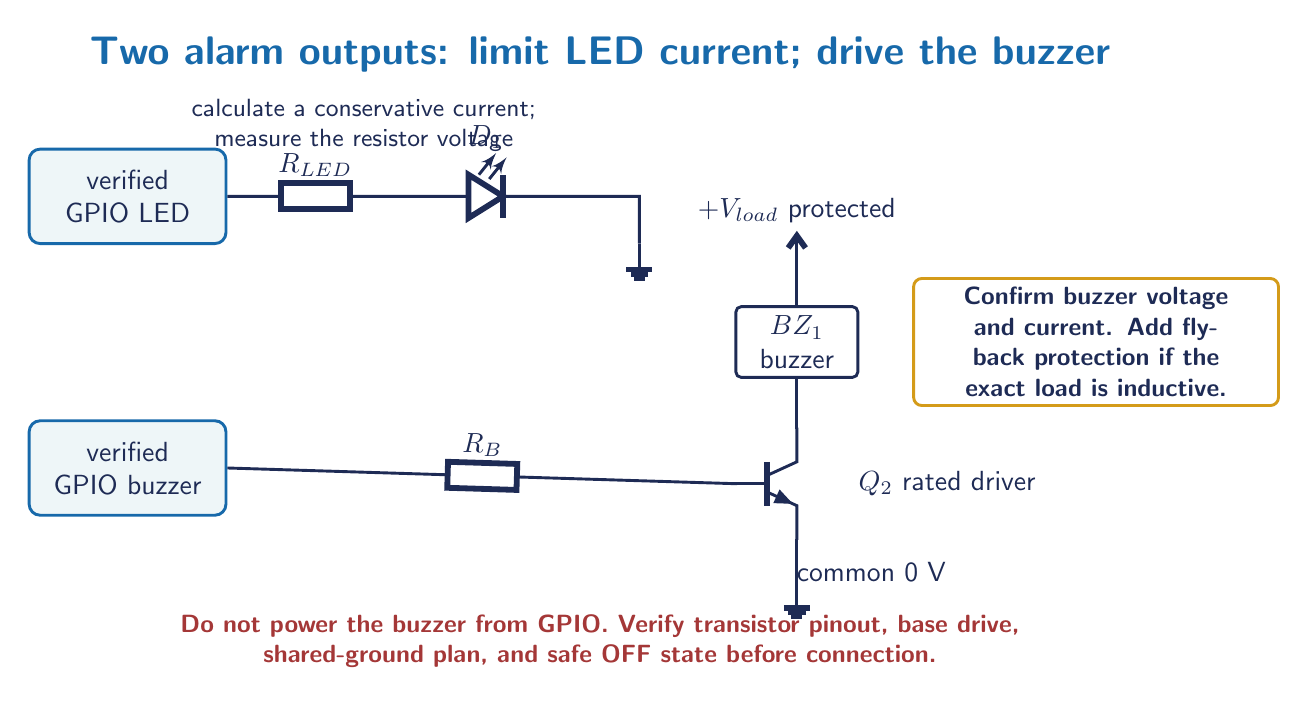
\begin{tikzpicture}[line width=1.05pt,draw=TEJNavy,text=TEJNavy,font=\sffamily]
  \ctikzset{bipoles/length=1.1cm}
  \node[font=\bfseries\Large,text=TEJBlue] at (7.5,7.0)
    {Two alarm outputs: limit LED current; drive the buzzer};

  % LED channel
  \node[draw=TEJBlue,rounded corners=4pt,fill=TEJLight,minimum width=2.5cm,minimum height=1.2cm,align=center]
    (gpioled) at (1.5,5.2) {verified\\GPIO LED};
  \draw (gpioled.east) to[R,l={$R_{LED}$}] (5.0,5.2)
    to[leD,l={$D_1$}] (7.1,5.2) -- (8.0,5.2) -- (8.0,4.6) node[ground] {};
  \node[font=\small,align=center] at (4.5,6.1)
    {calculate a conservative current;\\measure the resistor voltage};

  % Buzzer driver channel
  \node[draw=TEJBlue,rounded corners=4pt,fill=TEJLight,minimum width=2.5cm,minimum height=1.2cm,align=center]
    (gpiobuzz) at (1.5,1.75) {verified\\GPIO buzzer};
  \node[npn,scale=1.15] (q2) at (10.0,1.55) {};
  \draw (gpiobuzz.east) to[R,l={$R_B$}] (q2.B);
  \draw (q2.E) -- ++(0,-0.55) node[ground] {common 0 V};
  \node[draw=TEJNavy,rounded corners=2pt,minimum width=1.55cm,minimum height=0.9cm,align=center]
    (buzzer) at (10.0,3.35) {$BZ_1$\\buzzer};
  \draw (q2.C) -- (buzzer.south);
  \draw (buzzer.north) -- ++(0,0.55) node[vcc] {$+V_{load}$ protected};
  \node[anchor=west] at (10.65,1.55) {$Q_2$ rated driver};

  \node[draw=TEJGold,rounded corners=3pt,align=center,text width=4.4cm,font=\bfseries\small]
    at (13.8,3.35) {Confirm buzzer voltage and current. Add flyback protection if the exact load is inductive.};
  \node[text=TEJRed,font=\bfseries\small,align=center] at (7.5,-0.45)
    {Do not power the buzzer from GPIO. Verify transistor pinout, base drive,\\shared-ground plan, and safe OFF state before connection.};
\end{tikzpicture}
\end{document}
